\chapter{Trajectory Planning}%
\label{CH:PLANNING}

%----------------------------------------------------------------------------------------
\section{The Framework}
In the previous chapter, we tracked the problem of autonomous environment \emph{exploration} from a very practical point of view,
providing a couple of possible solutions to efficiently compute high informative trajectories. Here, we moved to a slightly different
problem as the environment to navigate is completely known and the main objective is to move the autonomous agent from an initial
position, to a final one, without getting in collision with the mapped obstacles and without the necessity to gather information about
the surroundings. In these settings, the planned trajectory is required only to be \emph{safe} in the sense that does not collide with
any obstacles and develops inside known and free environment areas, and to fully satisfy the agent dynamical capabilities.
As the trajectory is not meant to gather as much data as possible, it can be designed to optimise whatever user-defined loss function,
from the overall travel time, to control effort, or high derivatives. In the Leonardo drone contest case, a trajectory planning module
was required to navigate the environment and reach a goal position smoothly and quickly, so the quadrotor is steered in a way that
the localisation and the collision avoidance (see later in~\chref{CH:AVOIDANCE}) parts can work as well as possible.

In this chapter, after a brief literature review, we analyze and adapt a state-of-the-art solution to the trajectory planning problem.
The proposed solution has been successfully implemented and deployed during the Leonardo drone contest.
For further details the reader is referred to the original work~\cite{zhou2019robust}.

\subsection{Related Works}
Although the literature is cluttered with possible solutions to the problem of trajectory planning, most of them can be classified
solely into two categories: \emph{hard-constrained} and \emph{soft-constrained} methods.
Hard-constrained methods reformulate the planning problem as a convex optimisation one, where collisions are avoided by constraining
the planned path to be inside a set of convex flight corridors.
This idea was pioneered by~\cite{mellinger2011minimum} who proposes to generate minimum-snap trajectories
via Quadratic Programming (QP) approach, and by~\cite{richter2016polynomial} who, in turn, presented a closed-form approach
to the minimum-snap trajectory generation problem.
Both the latter approaches parametrise the overall trajectory as $n$-segments piecewise polynomial curve,
and ensure the trajectory safety by iteratively adding intermediate waypoints.
Similar approaches generate safe trajectories via convex optimisation~\cite{chen2015real, gao2016online, liu2017planning, ding2018trajectory, ding2019efficient, gao2018online},
but, unlike the pioneer solutions, here the problem is solved in a two-steps pipeline. First, a sequence of cubes~\cite{gao2018online},
spheres~\cite{gao2019flying}, or polyhedrons~\cite{liu2017planning}, are fitted inside the free and navigable space, then the
reconstructed flight corridors are used as convex constraints inside the optimisation problem.
The works of~\cite{ding2018trajectory, ding2019efficient} proposed a B-Spline-based search able to generate trajectories used as 
an initial guess for the subsequent optimisation step.
Thanks to the convex reformulation, hard-constrained methods guarantee global optimality at the expense of all possible nonconvex
costs and constraints, such as distance from obstacles and conservative kinodynamic constraints, leading often to unsafe and
conservative paths.
On the other hand, soft-constrained methods reformulate trajectory planning as a non-linear optimisation problem able to keep
smoothness, feasibility, and safety into account.
In~\cite{zucker2013chomp} the authors generate discrete-time trajectories minimizing both smoothness and risk of collision via
gradient descent methods, while in~\cite{kalakrishnan2011stomp} the optimisation is solved in a gradient-free fashion.
The work of~\cite{oleynikova2016continuous} extended the latter approaches to continuous-time polynomial trajectories, thanks to the
continuous-time formulation it avoids numeric differentiation errors leading to a more accurate representation.
However, the approach proposed by~\cite{oleynikova2016continuous} suffers from low success rate, being the proposed optimisation problem
solved without a good initial guess.
As a matter of fact, the success rate considerably improved when~\cite{gao2017gradient} proposes to solve the same problem
with a collision-free path used as an initial condition. The latter path is obtained via sampling-based path searching methods.
In~\cite{usenko2017real} the trajectory is parameterized as an uniform B-Spline, whose intrinsic continuity allows to reduce
the overall number of constraints.
Soft-constrained solutions make use of gradient information to push the final trajectory far from obstacles, but may suffer from
local minima and do not have any guarantee of success rate and kinodynamic feasibility.
The work of~\cite{zhou2019robust} proposes a novel soft-constrained method where the B-Spline parameterisation is used to both
speed-up the cost computation and simplify the collision checking thanks to its convex hull containment property (see~\appref{SEC:SPLINES-APPENDIX}).

%----------------------------------------------------------------------------------------
\section{Quadrotor Trajectory Generation}
In this section we review a trajectory planning approach first proposed by~\cite{zhou2019robust}.
The considered approach aims to efficiently compute minimum effort safe trajectories, balancing both the induced control effort and
the overall trajectory time. This soft-constrained approach develops in two steps, first a collision-free suboptimal trajectory
is computed via \emph{hybrid-state} A$^{\star}$ search, then the obtained solution is iteratively refined via non-linear
optimisation. In this second step the B-Spline formulation is adopted to improve the algorithm convergency rate.

\subsection{Hybrid-State A$^{\star}$}
The first step consists of raw trajectory planning via A$^{\star}$ graph search, unlike the standard A$^{\star}$ formulation, here
the proposed solution expands and optimises a graph of possible kinodynamic feasible trajectories (from this property the \emph{hybrid-state} attribute).
In this settings, the A$^{\star}$ optimisation is applied to a tree $\tree = \lp \NN, \EE \rp$ consisting of a set of nodes
$\NN = \left\{ N_1, \dots, N_{n_{N}} \right\}$ and a set of edges $\EE = \left\{ E_1, \dots, E_{n_{E}} \right\}$, where each node
is completely defined by the following six quantities
\begin{equation*}
	\NN_i = \left\{ \bs{x}_i, \bs{u}_i, \delta^t_i, \chi_i, g_i, h_i \right\},
\end{equation*}
where $\bs{x}_i$ and $\bs{u}_i$ represent the current quadrotor state and the applied input used to reach that state,
$\delta^t_i$ is the amount of time for which $\bs{u}_i$ is applied, $\chi_i$ is an unique integer indexing $\bs{x}_i$ over a voxel grid,
and $\lp g_i, h_i \rp$ are two costs associated with the current node useful for the graph optimisation, in particular $g_i$ is the
\emph{true} trajectory cost, while $h_i$ represents a heuristic estimating the cost-to-go to reach the goal state.
The graph edges are generated by motion primitives respecting the quadrotor dynamics, instead of standard straight lines.
As in~\secref{SEC:EXPLORATION-LARGE-SCALE}, here we enforce the differential flatness property commonly used in quadrotor planning,
and express the final state trajectory through the evolution of only the three axis-wise positions
so $\bs{x} = \lp p_x, p_y, p_z \rp \in \R^3$, where each component can be designed as a time-parameterized polynomial function
\begin{equation}
	\label{EQ:POLYNOMIAL-EXPANSION}
	p_j \lp t \rp = \sum_{k=0}^{n} a_kt^k.
\end{equation}
The aformentioned formulation correspond to a Linear Time-Invariant (LTI) system, letting
$\bs{z} = \lp \bs{x}\T, \bs{x}^{{\lp 1 \rp}\T}, \dots, \bs{x}^{{\lp n-1 \rp}\T} \rp\T \in \R^{3n}$  the state vector,
and $\bs{u} =  \bs{x}^{\lp n \rp} \in \mathcal{U} = \lps \bs{u}_{\text{min}}, \bs{u}_{\text{max}}\rps \subset \R^{3}$ the control input,
then the state-space model can be defined as
\begin{equation*}
	\dot{\bs{z}} = A \bs{z} + B \bs{u},
\end{equation*}
with $A \in \R^{3n \times 3n}$ and $B \in \R^{3n \times 3}$ matrices in prime form.
The complete solution for the state equation, giving the quadrotor trajectory from the initial condition $\bs{z}_0$, is expressed as
\begin{equation}
	\label{EQ:MOTION-PRIMITIVE}
	\bs{z}\lp t \rp = \exp \lp At \rp\bs{z}_0 + \int_{0}^{t} \exp \lp A \lp t-\tau \rp \rp B \bs{u}\lp \tau \rp d\tau.
\end{equation}
In these settings, a set of motion primitive, leading to a set of possible graph edges for each node, can be efficiently computed
by propagating~\eqqref{EQ:MOTION-PRIMITIVE} for a fixed time step $\delta^t$, applying a set of discretised control inputs
$\mathcal{U}_{\text{D}} \subset \mathcal{U}$. From a practical point of view, the set $\lps \bs{u}_{\text{min}}, \bs{u}_{\text{max}} \rps$
can be uniformly discretised in $r$ steps along each axis, yielding to $r^3$ possible motion primitives.
The graph search then unfolds as a classical A$^{\star}$ search, for each node a set of edges and children nodes are generated via motion
primitive propagation, then each child is checked against dynamical feasibility and possible collision with map obstacles, and only those
nodes considered as feasible are retained for future expansions.
To speed-up the search a voxel grid discretisation is imposed over the trajectory space so all children nodes whose associated index $\chi$
matches in the list of already expanded cells are culled out from the open set.

In order to let the adopted search effective, we need an admissible and informative loss formulation for both the true trajectory cost
and the estimated cost-to-go. Under this perspective, since the main trajectory planning objective is to generate motions balancing both
control effort and overall traveling time, the natural loss formulation is
\begin{equation}
	\label{EQ:PLANNING-LOSS}
	\loss = T + \rho \int_0^T \norm{\bs{u} \lp \tau \rp}^2 d \tau,
\end{equation}
where $T$ is the total trajectory time, $\bs{u}$ is the control action, and $\rho \in \R_{>0}$ is a weight coefficient balancing between
minimum time and minimum effort trajectories.
Under the loss function~\eqref{EQ:PLANNING-LOSS}, the true cost $g_i$, representing the trajectory cost form the start position, can be
computed summing up the cost of all primitives applied so far
\begin{equation*}
	g_i = g_{i-1} + \lp 1 + \rho\norm{\bs{u}_i}^2 \rp \delta_i^t.
\end{equation*}
As regards the heuristic cost-to-go $h_i$, we need an estimation of $\loss$ from the current state $\bs{x}_i$ to the goal one.
To retrieve this estimation, we compute a closed-form trajectory, from $\bs{x}_i$ to the goal state, that minimizes the cost $\loss$
by applying the Pontryagins minimum principle~\cite{mueller2015computationally}.
In particular, letting $n = 3$ in~\eqqref{EQ:POLYNOMIAL-EXPANSION}, then the optimal trajectory $p\lp t \rp$ minimising $\loss$ can
be computed as
\begin{equation}
	\label{EQ:OPTIMAL-TRAJECTORY}
	p^{\star}_{\mu} = \frac{1}{6}\alpha_{\mu}t^3 + \frac{1}{2}\beta_{\mu}t^2 + v_{\mu_0}t + p_{\mu_0} \hspace*{0.5cm} \text{with } \mu = x,y,z,
\end{equation}
where the parameters $\alpha_{\mu}$ and $\beta_{\mu}$ follow the relation
\begin{equation*}
	\begin{pmatrix}
		\alpha_{mu} \\ \beta_{\mu}
	\end{pmatrix} = \frac{1}{T^{{\star}^3}}
	\begin{pmatrix}
		-12 & 6T^{\star} \\ 6T^{\star} & -12T^{{\star}^2}
	\end{pmatrix}
	\begin{pmatrix}
		p_{\mu_{\text{goal}}} - p_{\mu_0} - v_{\mu_{\text{goal}}}T^{\star} \\
		v_{\mu_{\text{goal}}} - v_{\mu_{0}}
	\end{pmatrix},
\end{equation*}
and $p_{\mu_0}$, $p_{\mu_{\text{goal}}}$, $v_{\mu_0}$, and $v_{\mu_{\text{goal}}}$ represent the initial and goal position and velocity, respectively.
The optimal time $T^{\star}$ can be compute by deriving~\eqqref{EQ:OPTIMAL-TRAJECTORY} and plugging it inside~\eqqref{EQ:PLANNING-LOSS}
\begin{equation*}
	T^{\star} = \argmin_{T > 0} \sum_{\mu \in \{ x,y,z \}} \frac{1}{3} \alpha_{\mu}^2T^3 + \alpha_{\mu}\beta{\mu}T^2 + \beta_{\mu}^2T.
\end{equation*}
The optimal cost $\loss^{\star} = \loss \lp p^{\star}, T^{\star}\rp$ is then used in place of $h_i$ as cost-to-go estimation.
\begin{remark}
	The choice $n = 3$ leads to \emph{minimum jerk} trajectories as the control action $\bs{u} = \bs{x}^{\lp 3 \rp}$. 
\end{remark}
\begin{remark}
	The computed optimal trajectory $p^{\star}$ contributes to the planning procedure more than only providing an admissible heuristic.
	As a matter of fact, $p^{\star}$ is useful twice as it can be used to stop the search in advance, provided that the computed trajectory
	satisfies all dynamical and collision constraints. Moreover, such an analytic expansion is of fundamental importance as, due to the
	control discretisation, it is difficult to have a primitive end exactly in the goal state.
\end{remark}

\subsection{B-Spline Trajectory Optimisation}
The second step of the proposed trajectory planning method consists of a trajectory optimisation procedure.
This step is fundamental in smoothing the initial trajectory produced by the path searcher, which is suboptimal due to the control discretisation,
and to push the final trajectory away from the obstacles, since the distance information in the free space is ignored at search time.
Here, as in~\secref{SEC:SEARCH-TRAJECTORY-OPTIMISATION}, to speed-up the solver and improve the planner success rate, we enforce the use of
B-Spline curves (see~\secref{SEC:SPLINES-APPENDIX}) as time parameterisation for the quadrotor trajectory.
As already mentioned in~\secref{SEC:SEARCH-TRAJECTORY-OPTIMISATION}, B-splines are defined by a set of control points
$\CP = \lps \bs{\cpoint}_0, \dots, \bs{\cpoint}_{\cpnumber} \rps$, and a set of time knots
$\bs{\splinevar} = \lps \splinevar_0, \dots, \splinevar_{\cpnumber + \order + 1} \rps$, as
\begin{equation*}
	\bs{\spline} \lp \splinevar \rp = \sum_{i=0}^\cpnumber \basis_i^\order \lp \splinevar \rp \bs{\cpoint}_i,
\end{equation*}
with $\order$ order of the spline and $\basis_i^\order$ basis functions, recursively computed via the De-Boor formula~\cite{de1978practical}.
The use of B-Spline in trajectory optimisation is attractive thanks to its convex hull containment property, which allows approximating
the collision condition of the overall trajectory by directly conditioning its control points $\CP$ lying to a free non-necessary convex
environment area. Moreover, by evaluating the control points distance from the obstacles we can directly assess the trajectory safeness.
Another useful property is represented by the closure with respect to integration and derivation, so the derivatives $\bs{\spline}^{\lp d \rp}$
of a B-Spline still maintain a B-Spline structure with control points
\begin{equation*}
	\bs{\cpoint}_i^{\lp d \rp} = \order \frac{\bs{\cpoint}_{i+1}^{\lp d-1 \rp} - \bs{\cpoint}_i^{\lp d-1 \rp}}{\splinevar^{\lp d-1 \rp}_{i+\order+1} - \splinevar^{\lp d-1 \rp}_{i+1}}.
\end{equation*}
These properties, jointly with the differential flatness one, can be used to ease the trajectory optimisation procedure as both the
collision and dynamics constraints can be refurmulated linearly in terms of the trajectory control points, which are then used as
decision variables. For this purpose, we fix an uniformly distributed knot vector of the form
\begin{equation*}
	\bs{\splinevar} =
	\begin{bmatrix}
		0_{0:7}, & \Delta_{\splinevar}, & 2\Delta_{\splinevar}, & \dots, & (\cpnumber-\order)\Delta_{\splinevar}, & T_{0:7}
	\end{bmatrix},
\end{equation*}
with $\Delta_{\splinevar} = T/(\cpnumber - \order + 1)$, and $T$ the total trajectory time computed in the search phase.
Then we formulate the trajectory optimisation step as an uncostrained optimisation problem of the form
\begin{equation}
	\label{EQ:PLANNING-OPTIMISATION}
	\min_{\bs{\cpoint}_0, \bs{\cpoint}_1, \dots, \bs{\cpoint}_{\cpnumber}} \lambda_{\text{s}} \loss_{\text{s}} + 
	\lambda_{\text{c}} \loss_{\text{c}} + \lambda_{\text{f}} \lp \loss_{\text{v}} + \loss_{\text{a}} \rp,
\end{equation}
where $\lambda_{\text{s}} \in \R_{<0}$, $\lambda_{\text{c}} \in \R_{<0}$, and $\lambda_{\text{f}} \in \R_{<0}$ are
weight coefficients balacing between trajectory smoothness $\loss_{\text{s}}$, distance from obstacles $\loss_{\text{c}}$,
velocity feasibility $\loss_{\text{v}}$, and acceleration feasibility $\loss_{\text{a}}$.
Each cost is formulated taking into account the B-Spline parameterisation and properties.
The smoothness cost $\loss_{\text{s}}$ tries to pursue the same goal carried out by the searcher to minimise the overall control
effort, thus with $n = 3$, $\loss_{\text{s}}$ reads to
\begin{equation*}
	\loss_{\text{s}} = \int_0^{T} \norm{\frac{d^n \bs{\spline} \lp \splinevar \rp}{d \splinevar^n}}^2 d \splinevar,
\end{equation*}
which can be computed in closed form for B-Spline parameterisation (see~\secref{SEC:SPLINES-APPENDIX}).
The collision cost $\loss_{\text{c}}$ is formulated as the repulsive force of the obstacles acting on each control point
\begin{equation*}
	\loss_{\text{c}} = \sum_{i = 0}^{\cpnumber}
	\begin{cases}
		\begin{matrix}
			\lp d \lp \bs{\cpoint}_i \rp - d_{\text{thr}} \rp^2 & d \lp \bs{\cpoint}_i \rp \le d_{\text{thr}}, \\
			0 & d \lp \bs{\cpoint}_i \rp > d_{\text{thr}},
		\end{matrix}
	\end{cases}
\end{equation*}
where $d \lp \bs{\cpoint}_i \rp$ is the distance of $\bs{\cpoint}_i$ from the closer mapped obstacle, and $d_{\text{thr}}$
is a minimum distance considered as \emph{safe}.
Finally the velocity and acceleration feasibility cost is formulated as
\begin{equation*}
	\loss_{\text{v}} = \sum_{\mu = \{ x,y,z \}} \sum_{i = 0}^{\cpnumber - 1}
	\begin{cases}
		\begin{matrix}
			\lp \bs{\cpoint}_i^{{\lp 1 \rp}^2} - v_{\text{max}}^2 \rp^2 & \bs{\cpoint}_i^{{\lp 1 \rp}^2} \le v_{\text{max}}^2, \\
			0 & \bs{\cpoint}_i^{{\lp 1 \rp}^2} < v_{\text{max}}^2,
		\end{matrix}
	\end{cases}
\end{equation*}
\begin{equation*}
	\loss_{\text{a}} = \sum_{\mu = \{ x,y,z \}} \sum_{i = 0}^{\cpnumber - 2}
	\begin{cases}
		\begin{matrix}
			\lp \bs{\cpoint}_i^{{\lp 2 \rp}^2} - a_{\text{max}}^2 \rp^2 & \bs{\cpoint}_i^{{\lp 2 \rp}^2} \le a_{\text{max}}^2, \\
			0 & \bs{\cpoint}_i^{{\lp 2 \rp}^2} < a_{\text{max}}^2,
		\end{matrix}
	\end{cases}
\end{equation*}
where $v_{\text{max}}$ and $a_{\text{max}}$ are the axis-wise maximum velocity and acceleration, respectively.
\begin{remark}
	The problem~\eqref{EQ:PLANNING-OPTIMISATION} does not ensure neither safety, nor dynamical feasibility as the constraints
	has been softly injected inside the cost. Nevertheless, there exists a local optimal close to the initial trajectory planned by
	the searcher, so the problem~\eqref{EQ:PLANNING-OPTIMISATION} quickly converges to the local optimal solution if initialised with a
	good and feasible initial condition.
\end{remark}

\subsection{Experimental Results}
\begin{figure}[!t]
	\begin{center}
		\begin{minipage}{.45\linewidth}
			\centering
			\subfloat[]{%
				\label{FIG:PLANNING-RESULTS-MAP-TRAJECTORY-A}%
				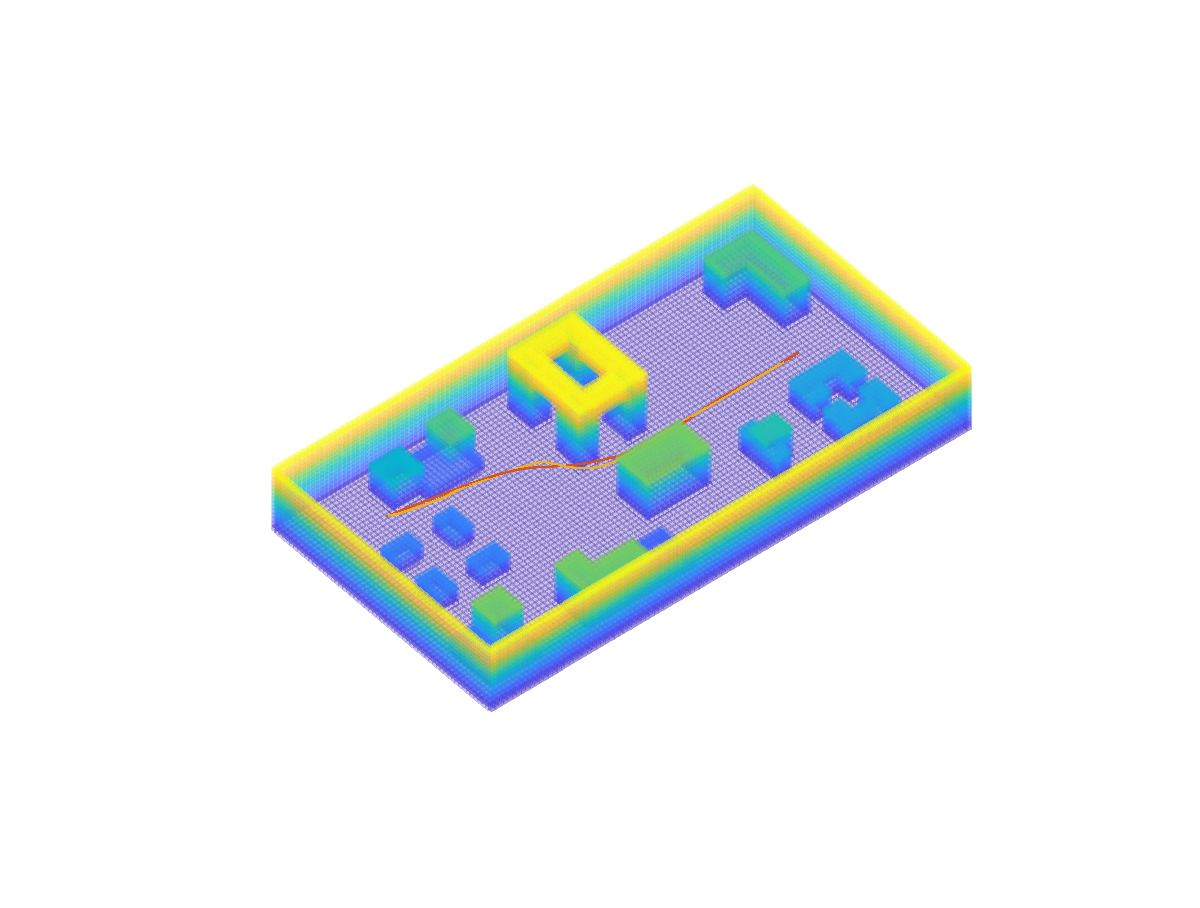
\includegraphics[trim={3.5cm 2.5cm 3cm 2.5cm}, clip = true, width = 1.05\textwidth]{Figs/Chapter5/planning-full.eps}}
		\end{minipage}
		\begin{minipage}{.45\linewidth}
			\centering
			\subfloat[]{%
				\label{FIG:PLANNING-RESULTS-MAP-TRAJECTORY-B}%
				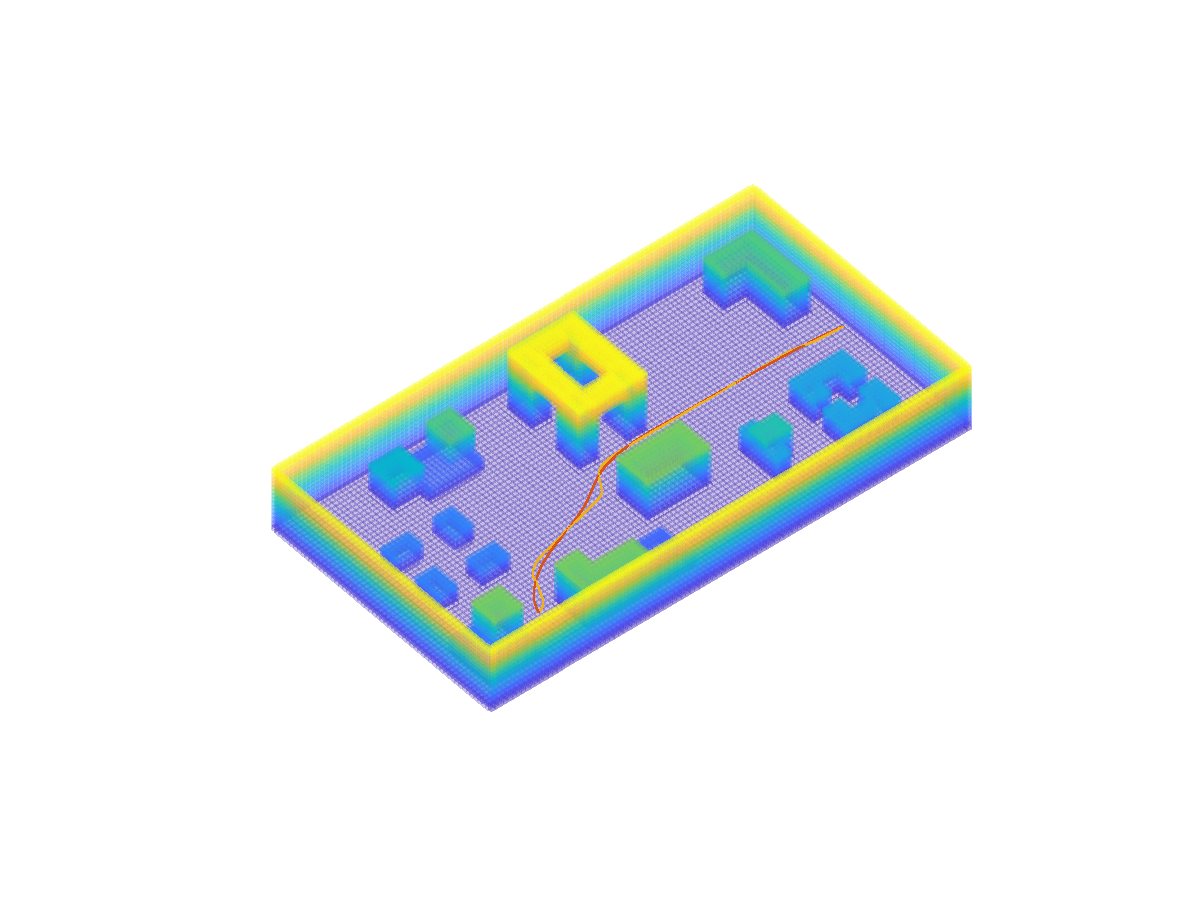
\includegraphics[trim={3.5cm 2.5cm 3cm 2.5cm}, clip = true, width = 1.05\textwidth]{Figs/Chapter5/planning-full-2.eps}}
		\end{minipage}
	\end{center}
	\caption{Results of the proposed trajectory planning algorithm. The figure depicts the simulated environment along with the planned
	trajectory by the searcher (yellow line), and the output of the trajectory optimisation step (red line). Notice how the optimised
	trajectory smoothly follows the yellow path without colliding with the environment obstacles.}%
    \label{FIG:PLANNING-RESULTS-MAP-TRAJECTORY}
\end{figure}
\begin{figure}[!t]
	\begin{center}
		\begin{minipage}{.45\linewidth}
			\centering
			\subfloat[]{%
				\label{FIG:PLANNING-RESULTS-TRAJECTORY-A}%
				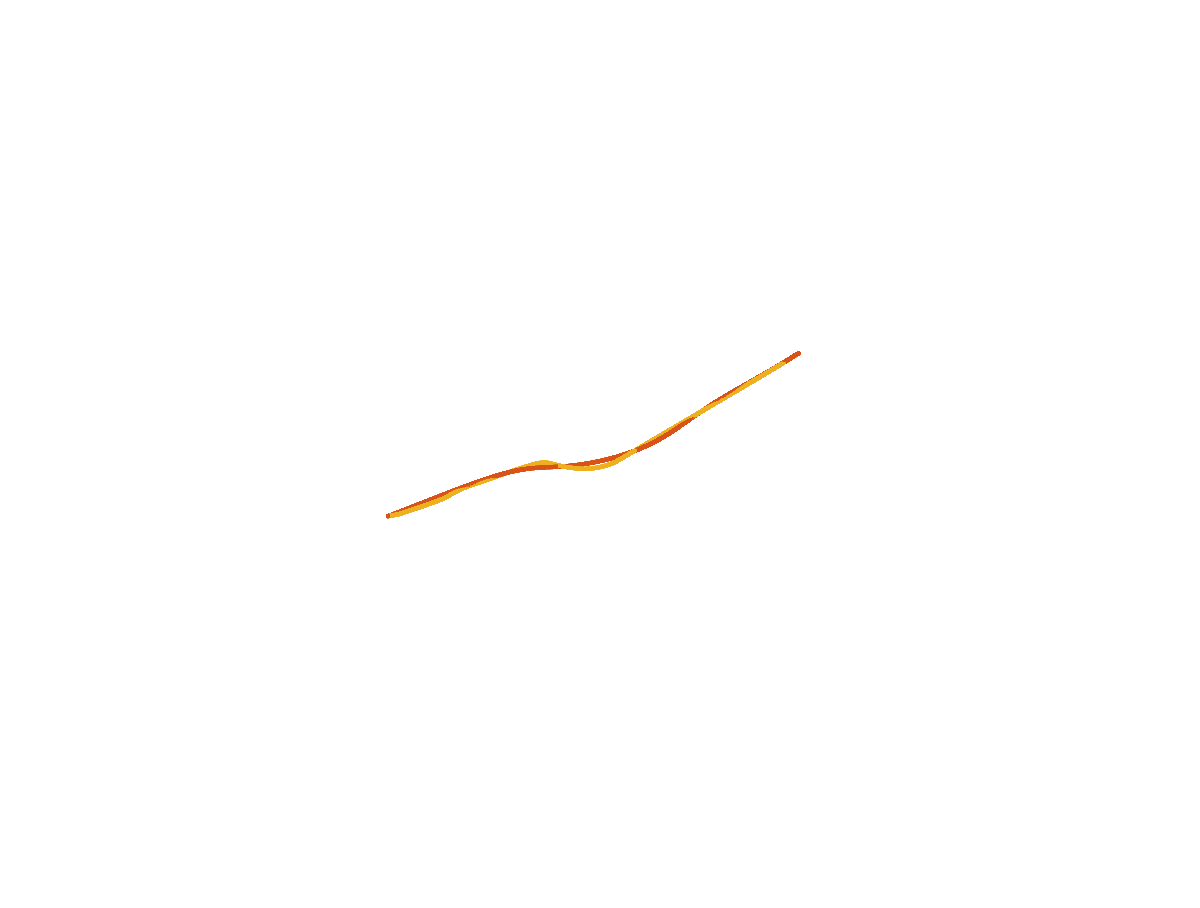
\includegraphics[trim={3.5cm 2.5cm 3cm 2.5cm}, clip = true, width = 1.05\textwidth]{Figs/Chapter5/planning-traj.eps}}
		\end{minipage}
		\begin{minipage}{.45\linewidth}
			\centering
			\subfloat[]{%
				\label{FIG:PLANNING-RESULTS-TRAJECTORY-B}%
				
\includegraphics[trim={3.5cm 2.5cm 3cm 2.5cm}, clip = true, width = 1.05\textwidth]{Figs/Chapter5/planning-traj-2.eps}}
		\end{minipage}
	\end{center}
	\caption{Results of the proposed trajectory planning algorithm. The picture reports the same results displayed in~\figref{FIG:PLANNING-RESULTS-MAP-TRAJECTORY}
	without the environment map for better visualisation.}%
    \label{FIG:PLANNING-RESULTS-TRAJECTORY}
\end{figure}
The results obtained applying the proposed approach are reported in Figures~\ref{FIG:PLANNING-RESULTS-TRAJECTORY-A} and~\ref{FIG:PLANNING-RESULTS-TRAJECTORY-B},
where the yellow lines represent the trajectories computed by the path searcher, while the red lines are the outputs of the trajectory optimisation step.
As the reader can observe, both yellow and red lines lie to the free part of the environment, ensuring safeness of the overall trajectory,
moreover the yellow path presents sharp turns which are not present in the red one.
This latter property is the smoothing effect introduced by the optimiser, that, unlike the search part,
makes use of a continuous set of possible inputs $\bs{u}$.

%----------------------------------------------------------------------------------------
\section{Contributions}
The chapter is devoted to discuss the problem of trajectory planning in completely known and mapped environments.
The discussion unfolds by first reviewing the current state-of-the-art solutions then we review and implement one of the most promising
approach to the problem of quadrotor trajectory planning in cluttered environments. The proposed solution has been deeply analyzed,
implemented, and deployed during the Leonardo drone contest with great results. Moreover, the implemented solution has been fully
integrated inside a complete navigation pipeline which makes use, and thus may be affected by noise and errors, of a localisation,
mapping, planning, replanning, and control pipeline. The implemented solution has been tested in a bunch of different scenarios where
the surrounding map was continuously kept updated and the planning procedure may, sometimes, not have a feasible solution.

%------------------------------------------------